\chapter{局部 Fourier 分析与两网格收敛分析}
\label{ch:lfa}

\begin{keybox}
\textbf{本章把前几章的全局谱认识推进到局部频率与 两网格 收敛分析。}
\chapref{ch:linear-solvers}已经建立一般线性求解与收敛语言，\chapref{ch:two-grid}则对一维 Poisson 算出 Jacobi 的网格依赖谱，并用高频放大因子建立平滑性质和粗空间校正。本章不重复“是否收敛”的基础结论，而是转向平移不变局部模型，用 Fourier 符号同时表示平滑器与粗网格校正，并完整算完一套一维两网格收敛因子。经典多重网格教材通常用 Fourier 模态解释平滑性质，而系统的局部 Fourier 分析进一步把限制、延拓和粗网格校正都写入小型符号矩阵中\cite{briggs2000,trottenberg2001,wienands2004}。

核心路线是
\[
\boxed{
\text{离散模板}
\rightar行
\text{Fourier 符号}
\rightar行
\text{谐波对}
\rightar行
2\times2\text{ 两网格符号}
\rightar行
\rho_{TG}.}
\]
一维先完整承担决定 两网格 收敛的代数步骤；二维与三维随后只扩展频率空间几何和 谐波子空间 的维数。
\end{keybox}

\section{Fourier 模态与离散符号}
\label{sec:lfa-fourier}

先把\chapref{ch:linear-solvers}里已经出现的误差形状统一写成频率表示。交替误差
\begin{equation}
e_j=(-1)^j=e^{\mathrm i\pi j}
\end{equation}
对应频率 $\theta=\pi$；缓慢变化的误差则对应 $|\theta|\ll1$。在均匀无限网格或周期网格上，使用复指数
\begin{equation}
\varphi_h(\theta;j)=e^{\mathrm i j\theta},
\qquad
\theta\in[-\pi,\pi)
\label{eq:lfa-fourier-mode}
\end{equation}
最方便，因为正弦和余弦只是其实部与虚部。

若一个平移不变离散算子 $A_h$ 满足
\begin{equation}
A_h\varphi_h(\theta)
=\widetilde A_h(\theta)\varphi_h(\theta),
\end{equation}
则乘数 $\widetilde A_h(\theta)$ 称为 $A_h$ 的\textbf{Fourier 符号}。这个符号并不是额外定义出来的经验函数，而是把复指数模态代入离散模板以后自然得到的特征值。

设一般一维常系数模板写成
\begin{equation}
(A_hu)_j
=
\sum_{m=-p}^{q}a_m u_{j+m}.
\label{eq:lfa-general-stencil}
\end{equation}
代入
\begin{equation}
u_{j+m}
=
e^{\mathrm i(j+m)\theta}
=
e^{\mathrm im\theta}\varphi_h(\theta;j),
\end{equation}
便得到
\begin{align}
(A_h\varphi_h)_j
&=
\sum_{m=-p}^{q}a_m
e^{\mathrm im\theta}
\varphi_h(\theta;j).
\end{align}
因此
\begin{equation}
\boxed{
\widetilde A_h(\theta)
=
\sum_{m=-p}^{q}a_m e^{\mathrm im\theta}.
}
\label{eq:lfa-general-symbol-formula}
\end{equation}
也就是说，离散符号就是模板系数关于偏移量 $m$ 的离散 Fourier 变换。固定 $\theta$ 后，原来作用于整个网格向量的模板被压缩成一个标量；若粗网格混叠会耦合若干 Fourier 模态，则这个标量进一步提升为一个很小的矩阵\cite{wienands2004}。

\begin{figure}[htbp]
\centering
\begin{tikzpicture}[x=0.82cm,y=0.78cm,font=\small]
  \draw[->] (-0.2,0)--(7.0,0) node[right] {$j$};
  \draw[->] (0,-1.5)--(0,1.6);
  \draw[domain=0:6.3,samples=100,line width=0.9pt]
    plot (\x,{0.75*sin(deg(0.55*\x))});
  \foreach \x in {0,...,6}{
    \fill (\x,{0.75*sin(deg(0.55*\x))}) circle (1.5pt);
  }
  \node[anchor=west] at (7.1,0.8) {低频：相邻点变化缓慢};

  \begin{scope}[yshift=-3.5cm]
    \draw[->] (-0.2,0)--(7.0,0) node[right] {$j$};
    \draw[->] (0,-1.5)--(0,1.6);
    \draw[domain=0:6.3,samples=140,line width=0.9pt]
      plot (\x,{0.75*sin(deg(2.65*\x))});
    \foreach \x in {0,...,6}{
      \fill (\x,{0.75*sin(deg(2.65*\x))}) circle (1.5pt);
    }
    \node[anchor=west] at (7.1,0.8) {高频：相邻点快速交替};
  \end{scope}
\end{tikzpicture}
\caption{同一细网格上的低频与高频离散模态。这里“高/低”是相对于网格采样和后续粗化而言的，不是连续函数的绝对属性。}
\label{fig:lfa-low-high-modes}
\end{figure}

\begin{warningbox}
\textbf{LFA 分析的是平移不变局部模型。}
物理边界、AMR 粗细接口、强系数跳变和一般不规则几何都会破坏全局平移不变性。因此 LFA 最适合解释局部机制、筛选 平滑器/传递算子 参数和预测 渐近行为，而不能把无限或周期模型的 符号 直接当作完整有限域系统的精确谱。AMR 离散结构见\chapref{ch:amr-discretization}。
\end{warningbox}

\section{一维 Poisson 的加权 Jacobi 分析}

一维标准 Poisson 离散为
\begin{equation}
(A_hu)_j
=\frac{-u_{j-1}+2u_j-u_{j+1}}{h^2}.
\label{eq:lfa-poisson-1d}
\end{equation}
代入式~\eqref{eq:lfa-fourier-mode}：
\begin{align}
(A_h\varphi)_j
&=\frac{-e^{-\mathrm i\theta}+2-e^{\mathrm i\theta}}{h^2}\varphi_j\\
&=\frac{2-2\cos\theta}{h^2}\varphi_j.
\end{align}
因此
\begin{equation}
\widetilde A_h(\theta)
=\frac{2-2\cos\theta}{h^2}
=\frac4{h^2}\sin^2\frac\theta2.
\label{eq:lfa-poisson-1d-symbol}
\end{equation}

Weighted Jacobi 的误差传播算子为
\begin{equation}
S_\omega=I-\omega D^{-1}A_h,
\end{equation}
而 $D=2h^{-2}I$，所以
\begin{equation}
\widetilde S_\omega(\theta)
=1-\omega(1-\cos\theta).
\label{eq:lfa-wj-one-dimensional-symbol}
\end{equation}

对 $2h$ 粗化，低频基本区取
\begin{equation}
\Theta_{2h}=\left(-\frac\pi2,\frac\pi2\right],
\label{eq:lfa-1d-low-frequency-domain}
\end{equation}
而其余频率相对于 粗网格 已无法独立解析。若只考察 高频 set
\begin{equation}
\frac\pi2\le|\theta|\le\pi,
\end{equation}
则 $1-\cos\theta\in[1,2]$。因此 加权 Jacobi 的高频 minimax 问题为
\begin{equation}
\min_\omega\max_{\lambda\in[1,2]}|1-\omega\lambda|.
\end{equation}
令区间两端等幅反号，得到
\begin{equation}
1-\omega=-(1-2\omega),
\end{equation}
于是
\begin{equation}
\boxed{\omega_\star=\frac23},
\qquad
\boxed{\mu=\frac13}.
\label{eq:lfa-1d-jacobi-optimal}
\end{equation}
这里 $\mu$ 是 平滑因子。它说明一次最优 加权 Jacobi 会把最坏 高频 amplitude 至少压到原来的 $1/3$；当 $\theta\to0$ 时，$\widetilde S_\omega(\theta)\to1$，光滑误差几乎不动。

\section{一维粗化与谐波对}
\label{sec:lfa-1d-aliasing}

Two-grid LFA 与单独分析 平滑器 的关键差别，是 粗网格 会让不同 细网格 frequencies 发生 混叠。对 粗网格节点 $j=2I$，有
\begin{align}
\varphi_h(\theta;2I)
&=e^{\mathrm i2I\theta},\\
\varphi_h(\theta+\pi;2I)
&=e^{\mathrm i2I(\theta+\pi)}
=e^{\mathrm i2I\theta}.
\end{align}
因此 细网格 模态 $\theta$ 与 $\theta+\pi$ 在 $2h$ grid 上完全不可区分。

\begin{figure}[htbp]
\centering
\begin{tikzpicture}[x=1.15cm,y=0.9cm]
  \draw[->] (-4.6,0)--(4.8,0) node[right] {$\theta$};
  \draw[thick] (-2,0.12)--(-2,-0.12) node[below=4pt] {$-\pi/2$};
  \draw[thick] (2,0.12)--(2,-0.12) node[below=4pt] {$\pi/2$};
  \draw[thick] (-4,0.12)--(-4,-0.12) node[below=4pt] {$-\pi$};
  \draw[thick] (4,0.12)--(4,-0.12) node[below=4pt] {$\pi$};
  \draw[line width=2.2pt] (-2,0)--(2,0);
  \node[above] at (0,0.15) {$\Theta_{2h}$};
  \fill (1,0) circle (2.3pt) node[above right] {$\theta$};
  \fill (-3,0) circle (2.3pt) node[above left] {$\theta+\pi\pmod{2\pi}$};
  \draw[->,bend left=28] (0.85,0.45) to node[above] {同一 粗网格模态} (-2.85,0.45);
\end{tikzpicture}
\caption{一维 $2h$ 粗化 下的 混叠。每个基本低频 $\theta\in\Theta_{2h}$ 都与一个相差 $\pi$ 的 细网格 谐波 配对；粗网格 无法区分这两个模态。}
\label{fig:lfa-1d-aliasing-pair}
\end{figure}

所以对每个 $\theta\in\Theta_{2h}$，两网格算子 必须在二维子空间
\begin{equation}
\mathcal E_\theta
=\operatorname{span}\left\{
\varphi_h(\theta),
\varphi_h(\theta+\pi)
\right\}
\label{eq:lfa-1d-harmonic-space}
\end{equation}
中分析。单个 Fourier 模态 已经不再保持不变，但这两个 谐波 张成的子空间保持不变。

\section{完整的一维两网格 Fourier 分析}
\label{sec:lfa-complete-1d-two-grid}

现在完整算一遍标准组合。取
\begin{itemize}
\item 细网格算子：式~\eqref{eq:lfa-poisson-1d}的一维 Poisson；
\item 平滑器：加权 Jacobi，权重 $\omega$；
\item 限制：\chapref{ch:two-grid}的 节点型全加权；
\item 延拓：节点型线性插值；
\item 粗网格算子：Galerkin $A_H=RA_hP$；
\item 平滑 次数：一次 pre-平滑 与一次 post-平滑。
\end{itemize}
这套选择不是 两网格 的定义，而是一个可以从头算完、并作为以后多维与复杂算子的参照模型。

令
\begin{equation}
c=\cos\theta,
\qquad
\alpha=\frac{1+c}{2},
\qquad
\beta=\frac{1-c}{2},
\label{eq:lfa-alpha-beta}
\end{equation}
于是 $\alpha+\beta=1$，且
\begin{equation}
4\alpha\beta=1-c^2=\sin^2\theta.
\end{equation}

\subsection{细网格算子与平滑器的谐波符号}

在基
\begin{equation}
\left\{
\varphi_h(\theta),
\varphi_h(\theta+\pi)
\right\}
\end{equation}
下，细网格 Poisson 算子 不耦合这两个 谐波，因此 符号 是对角矩阵。因为
\begin{align}
\widetilde A_h(\theta)
&=\frac{2(1-c)}{h^2}=\frac{4\beta}{h^2},\\
\widetilde A_h(\theta+\pi)
&=\frac{2(1+c)}{h^2}=\frac{4\alpha}{h^2},
\end{align}
所以
\begin{equation}
\widetilde A_h^{(2)}(\theta)
=\frac4{h^2}
\begin{b矩阵}
\beta&0\\
0&\alpha
\end{b矩阵}.
\label{eq:lfa-pair-fine-operator}
\end{equation}

Weighted Jacobi 同样是对角的：
\begin{equation}
\widetilde S_\omega^{(2)}(\theta)
=\begin{b矩阵}
s_0&0\\
0&s_1
\end{b矩阵},
\label{eq:lfa-pair-smoother}
\end{equation}
其中
\begin{align}
s_0
&=1-\omega+\omega c,\\
s_1
&=1-\omega-\omega c.
\label{eq:lfa-pair-smoothing-factors}
\end{align}
下标 $0,1$ 只表示 谐波对 中的两个分量，不表示 multigrid level。

\subsection{限制与延拓的谐波符号}

对 全加权
\begin{equation}
(Rr)_I
=\frac14r_{2I-1}+\frac12r_{2I}+\frac14r_{2I+1},
\end{equation}
作用于 $\varphi_h(\theta)$ 时，
\begin{align}
\widetilde R(\theta)
&=\frac14e^{-\mathrm i\theta}+\frac12+\frac14e^{\mathrm i\theta}\\
&=\frac{1+\cos\theta}{2}
=\alpha.
\end{align}
而对 paired 谐波，
\begin{equation}
\widetilde R(\theta+\pi)=\beta.
\end{equation}
因此从 谐波对 到唯一 粗网格模态 的 限制 符号 是行向量
\begin{equation}
\boxed{
\widetilde R^{(2)}(\theta)
=\begin{b矩阵}\alpha&\beta\end{b矩阵}.}
\label{eq:lfa-pair-restriction}
\end{equation}

延拓 的推导需要多一步。令 粗网格模态 为
\begin{equation}
\varphi_H(2\theta;I)=e^{\mathrm i2I\theta}.
\end{equation}
线性插值 后，偶数 细网格节点 保持 粗网格值，奇数 细网格节点 为相邻 粗网格值s 的平均：
\begin{align}
(P\varphi_H)_{2I}
&=e^{\mathrm i2I\theta},\\
(P\varphi_H)_{2I+1}
&=\frac12\left(e^{\mathrm i2I\theta}+e^{\mathrm i2(I+1)\theta}\right)\\
&=\cos\theta\;e^{\mathrm i(2I+1)\theta}.
\end{align}
把它写成两个 细层 谐波 的线性组合
\begin{equation}
P\varphi_H
=p_0\varphi_h(\theta)+p_1\varphi_h(\theta+\pi),
\end{equation}
在偶点与奇点分别比较系数：
\begin{equation}
p_0+p_1=1,
\qquad
p_0-p_1=\cos\theta.
\end{equation}
于是
\begin{equation}
\boxed{
\widetilde P^{(2)}(\theta)
=\begin{b矩阵}\alpha\\\beta\end{b矩阵}.}
\label{eq:lfa-pair-prolongation}
\end{equation}

这里 $\widetilde R^{(2)}$ 与 $\widetilde P^{(2)}$ 数值上看起来互为转置；它们来自\chapref{ch:two-grid}中 $R=\frac12P^T$ 的离散 传递算子，但 谐波 basis 的归一化已经吸收了网格点计数带来的缩放。

\subsection{Galerkin 粗网格算子}

粗网格频率 是 $2\theta$，且 $H=2h$。直接在 粗网格 上重新离散 Poisson 给出
\begin{align}
\widetilde A_H(2\theta)
&=\frac{2-2\cos(2\theta)}{H^2}\\
&=\frac{\sin^2\theta}{h^2}
=\frac{4\alpha\beta}{h^2}.
\label{eq:lfa-coarse-poisson-symbol}
\end{align}

Galerkin 计算给出同样结果：
\begin{align}
\widetilde R^{(2)}
\widetilde A_h^{(2)}
\widetilde P^{(2)}
&=
\begin{b矩阵}\alpha&\beta\end{b矩阵}
\frac4{h^2}
\begin{b矩阵}\beta&0\\0&\alpha\end{b矩阵}
\begin{b矩阵}\alpha\\\beta\end{b矩阵}\\
&=\frac{4\alpha\beta}{h^2}.
\end{align}
这就是附录~\ref{app:galerkin}逐点推导在 Fourier 空间中的压缩版本。

\subsection{粗网格校正的谐波矩阵符号}

由
\begin{equation}
C_h=I-PA_H^{-1}RA_h
\end{equation}
可得
\begin{align}
\widetilde C_h^{(2)}(\theta)
&=I-
\widetilde P^{(2)}
\widetilde A_H^{-1}
\widetilde R^{(2)}
\widetilde A_h^{(2)}\\
&=I-
\begin{b矩阵}\alpha\\\beta\end{b矩阵}
\begin{b矩阵}1&1\end{b矩阵}\\
&=
\boxed{
\begin{b矩阵}
\beta&-\alpha\\
-\beta&\alpha
\end{b矩阵}.}
\label{eq:lfa-coarse-correction-matrix}
\end{align}
这个矩阵有两个非常清楚的性质：
\begin{equation}
\widetilde C_h^{(2)}
\begin{b矩阵}\alpha\\\beta\end{b矩阵}=0,
\qquad
\widetilde C_h^{(2)}
\begin{b矩阵}1\\-1\end{b矩阵}
=\begin{b矩阵}1\\-1\end{b矩阵}.
\label{eq:lfa-coarse-correction-eigenvectors}
\end{equation}
第一式说明由 延拓 生成的 粗空间 分量 被精确消除；第二式说明 谐波对 中仍存在一个 粗网格 无法消除的互补方向。这正是\chapref{ch:two-grid}中 粗空间 投影 的频率域版本。

\subsection{两网格符号与收敛因子}

取一次 pre-平滑 与一次 post-平滑，并使用同一个 加权 Jacobi。由式~\eqref{eq:two_grid_error}，
\begin{equation}
\widetilde E_{TG}^{(2)}(\theta)
=
\widetilde S_\omega^{(2)}
\widetilde C_h^{(2)}
\widetilde S_\omega^{(2)}.
\end{equation}
代入式~\eqref{eq:lfa-pair-smoother}与~\eqref{eq:lfa-coarse-correction-matrix}：
\begin{equation}
\boxed{
\widetilde E_{TG}^{(2)}(\theta)
=
\begin{b矩阵}
\beta s_0^2&-\alpha s_0s_1\\
-\beta s_0s_1&\alpha s_1^2
\end{b矩阵}.}
\label{eq:lfa-two-grid-matrix-1d}
\end{equation}
其 determinant 为零，所以一个 特征值 恒为零；另一个 特征值 等于 trace：
\begin{align}
\lambda_{TG}(\theta;\omega)
&=\beta s_0^2+\alpha s_1^2\\
&=(1-\omega)^2
+\omega(3\omega-2)\cos^2\theta.
\label{eq:lfa-two-grid-nonzero-eigenvalue}
\end{align}

因此完整 两网格 收敛因子 不再需要猜测：
\begin{equation}
\rho_{TG}(\omega)
=\sup_{\theta\in\Theta_{2h}\setminus\{0\}}
\left|\lambda_{TG}(\theta;\omega)\right|.
\label{eq:lfa-two-grid-convergence-factor-1d}
\end{equation}
这里排除 $\theta=0$ 是因为无限/周期 Poisson 模型的 constant 模态 属于 null space；对非零频率取极限即可得到 supremum。

当 $\omega=2/3$ 时，式~\eqref{eq:lfa-two-grid-nonzero-eigenvalue}中的 $\cos^2\theta$ 系数恰好消失：
\begin{equation}
\boxed{
\lambda_{TG}\left(\theta;\frac23\right)=\frac19
\quad\text{for all }\theta\in\Theta_{2h}\setminus\{0\}.}
\label{eq:lfa-two-grid-one-ninth}
\end{equation}
所以这套标准 1D 两网格 组合的一次 循环 收敛因子为
\begin{equation}
\boxed{\rho_{TG}=\frac19.}
\end{equation}

这个结果比“Jacobi 的 平滑因子 是 $1/3$”更强：它把 平滑器、限制、延拓 与 粗网格求解 全部组合起来，得到完整 两网格 循环 的定量收缩率。

还可以反过来从式~\eqref{eq:lfa-two-grid-nonzero-eigenvalue}推导最优 $\omega$。由于 $\cos^2\theta\in[0,1)$，两端极限分别为
\begin{equation}
(1-\omega)^2,
\qquad
(1-2\omega)^2.
\end{equation}
最小化两者的最大值要求
\begin{equation}
|1-\omega|=|1-2\omega|,
\end{equation}
在 $1/2<\omega<1$ 内再次得到 $\omega=2/3$。这里 $2/3$ 不只是“高频平滑最优”，而且恰好使这套完整 一次预平滑/一次后平滑 两网格 组合的 收敛因子 达到 $1/9$。

\begin{checkpointbox}
取 $\theta=\pi/3$、$\omega=2/3$。此时 $\alpha=3/4$、$\beta=1/4$、$s_0=2/3$、$s_1=0$。直接代入式~\eqref{eq:lfa-two-grid-matrix-1d}，验证 两网格符号的非零特征值 为 $1/9$。这个手算例子可以独立检查上面的通式。
\end{checkpointbox}

\section{二维与三维的频率空间}

一维完整推导以后，再进入多维就可以清楚地区分“什么没有变”和“什么真正变了”。没有变的是 符号 思想与 两网格算子 的乘积结构；真正改变的是 高/低频区域的几何，以及 混叠谐波子空间 的维数。

二维 Fourier 模态 为
\begin{equation}
\varphi_{i,j}(\bm\theta)
=e^{\mathrm i(i\theta_x+j\theta_y)},
\qquad
\bm\theta=(\theta_x,\theta_y).
\end{equation}
二维五点 Poisson 的 符号 为
\begin{equation}
\widetilde A_h(\theta_x,\theta_y)
=\frac{4-2\cos\theta_x-2\cos\theta_y}{h^2},
\end{equation}
而
\begin{equation}
\widetilde{D^{-1}A}
=1-\frac12(\cos\theta_x+\cos\theta_y).
\label{eq:lfa-2d-dinv-a}
\end{equation}

对 $2h$ 全方向粗化，二维低频区域是
\begin{equation}
\Theta_{low}^{2D}
=\left(-\frac\pi2,\frac\pi2\right]^2,
\label{eq:lfa-2d-low-region}
\end{equation}
高频区域是整个 $[-\pi,\pi)^2$ 去掉这个中心方形后的补集。一个 模态 只要至少一个方向相对于 $2h$ grid 不可解析，就属于 高频 set。

\begin{figure}[htbp]
\centering
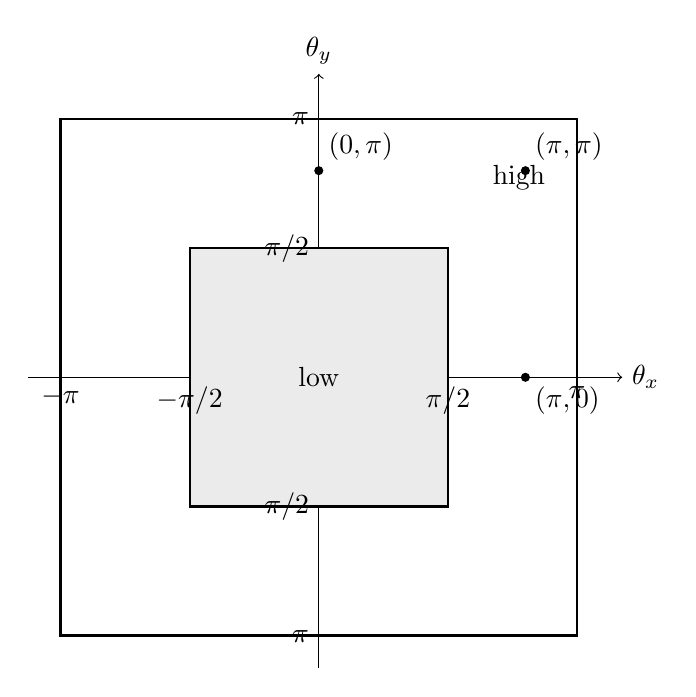
\begin{tikzpicture}[scale=0.82]
  \draw[->] (-4.5,0)--(4.7,0) node[right] {$\theta_x$};
  \draw[->] (0,-4.5)--(0,4.7) node[above] {$\theta_y$};
  \draw[thick] (-4,-4) rectangle (4,4);
  \fill[gray!16] (-2,-2) rectangle (2,2);
  \draw[thick] (-2,-2) rectangle (2,2);
  \node at (0,0) {low};
  \node at (3.1,3.1) {high};
  \node[below] at (-4,0) {$-\pi$};
  \node[below] at (-2,0) {$-\pi/2$};
  \node[below] at (2,0) {$\pi/2$};
  \node[below] at (4,0) {$\pi$};
  \node[left] at (0,-4) {$-\pi$};
  \node[left] at (0,-2) {$-\pi/2$};
  \node[left] at (0,2) {$\pi/2$};
  \node[left] at (0,4) {$\pi$};
  \fill (3.2,0) circle (2pt) node[below right] {$(\pi,0)$};
  \fill (0,3.2) circle (2pt) node[above right] {$(0,\pi)$};
  \fill (3.2,3.2) circle (2pt) node[above right] {$(\pi,\pi)$};
\end{tikzpicture}
\caption{二维 全方向粗化 的频率几何。中心方形是 粗网格 可独立表示的 低频 region；其补集都是 高频 模态。高频不是“两个方向都振荡”，而是至少一个方向落在 粗网格 无法解析的频率带。}
\label{fig:lfa-2d-frequency-region}
\end{figure}

在二维 高频 set 上，式~\eqref{eq:lfa-2d-dinv-a}覆盖区间 $[1/2,2]$。因此 point 加权 Jacobi 的高频 minimax 权重为
\begin{equation}
\omega_\star=\frac45,
\qquad
\mu_\star=\frac35.
\label{eq:lfa-2d-jacobi-optimal}
\end{equation}
这说明不能把一维 $\omega=2/3$ 当成与维数无关的常数。

三维 模态 为
\begin{equation}
\varphi_{i,j,k}(\bm\theta)
=e^{\mathrm i(i\theta_x+j\theta_y+k\theta_z)},
\end{equation}
并有
\begin{equation}
\widetilde{D^{-1}A}
=1-\frac13(
\cos\theta_x+\cos\theta_y+\cos\theta_z).
\end{equation}
低频区域变成 $(-\pi/2,\pi/2]^3$，高频 set 是其补集；对应 $\widetilde{D^{-1}A}$ 范围为 $[1/3,2]$，从而
\begin{equation}
\omega_\star=\frac67,
\qquad
\mu_\star=\frac57.
\label{eq:lfa-3d-jacobi-optimal}
\end{equation}

\section{多维谐波子空间与两网格符号}

二维 全方向粗化 时，$x,y$ 两个方向都存在“是否加 $\pi$”的二元选择。对基本低频 $\bm\theta=(\theta_x,\theta_y)$，粗网格 无法区分四个 细网格 谐波：
\begin{equation}
(\theta_x,\theta_y),\quad
(\theta_x+\pi,\theta_y),\quad
(\theta_x,\theta_y+\pi),\quad
(\theta_x+\pi,\theta_y+\pi).
\label{eq:lfa-two-dimensional-harmonics}
\end{equation}
因此 两网格符号 从一维的 $2\times2$ 扩展为四维 谐波子空间 上的 $4\times4$ 矩阵。三维三个方向各有一次二元 混叠 选择，共得到 $2^3=8$ 个 谐波，对应 $8\times8$ 符号。

由\chapref{ch:two-grid}式~\eqref{eq:two_grid_error}，任意维数的 两网格符号 都保持同一乘积结构：
\begin{equation}
\widetilde E_{TG}(\bm\theta)
=
\widetilde S_{\mathrm{post}}^{\nu_2}
\left[
I-\widetilde P
\widetilde A_H^{-1}
\widetilde R
\widetilde A_h
\right]
\widetilde S_{\mathrm{pre}}^{\nu_1}.
\label{eq:lfa-general-two-grid-symbol}
\end{equation}
只是这里的 $\widetilde A_h$、$\widetilde S$ 变成 $2^d\times2^d$ 矩阵，$\widetilde P$ 是 $2^d\times1$ 列，$\widetilde R$ 是 $1\times2^d$ 行，而 $\widetilde A_H$ 仍对应唯一 粗网格谐波。

最终 两网格 收敛因子 定义为
\begin{equation}
\rho_{TG}
=\sup_{\bm\theta\in\Theta_{low}}
\rho\left(\widetilde E_{TG}(\bm\theta)\right).
\label{eq:lfa-general-two-grid-factor}
\end{equation}
因此评价 平滑器 时必须回到完整组合：单独的 平滑因子 很重要，但它不能替代 $R/P$、粗网格算子 与 粗空间 approximation 对最终 $\rho_{TG}$ 的共同影响。

\section{Chebyshev 多项式平滑器}

前面的 符号 分析提供了理解 Chebyshev 平滑器 所需的谱语言。Weighted Jacobi 用一次线性多项式
\begin{equation}
1-\omega\lambda
\end{equation}
压低目标谱区；Chebyshev 平滑器 则构造更高阶多项式，使其在预先估计的高频 特征值 interval 上具有更小的最大幅值。

实现上，它主要由重复 算子应用、vector update 与少量 scalar recurrence 组成，不需要 Gauss--Seidel 那样的 pointwise ordering dependency，因此适合 GPU 与大规模 MPI。代价是需要估计目标谱区，而且一次 平滑 phase 包含多次 算子应用。评价标准仍然是
\begin{equation}
\text{达到目标精度的时间}
=\text{循环s}\times\text{cost per 循环},
\end{equation}
而不是只看某一步理论 放大因子\cite{baker2011smoothers,bergervergiat2021twostage,hypreBoomer2026}。

\section{各向异性与半粗化}

前面的一维完整推导与多维点 Jacobi 分析都依赖一个隐含条件：粗空间与平滑器的分工必须匹配算子的强耦合方向。考虑
\begin{equation}
-\epsilon u_{xx}-u_{yy}=f,
\qquad
0<\epsilon\ll1.
\label{eq:lfa-anisotropic-model}
\end{equation}
在各向同性网格 $h_x=h_y=h$ 上，标准五点离散的符号为
\begin{equation}
\boxed{
\widetilde A_h(\theta_x,\theta_y)
=
\frac4{h^2}
\left[
\epsilon\sin^2\frac{\theta_x}{2}
+
\sin^2\frac{\theta_y}{2}
\right].
}
\label{eq:lfa-anisotropic-symbol}
\end{equation}
对角部分为
\begin{equation}
D=\frac{2(\epsilon+1)}{h^2}I,
\end{equation}
所以
\begin{equation}
\widetilde{D^{-1}A}
=
\frac{2}{
1+\epsilon
}
\left[
\epsilon\sin^2\frac{\theta_x}{2}
+
\sin^2\frac{\theta_y}{2}
\right].
\label{eq:lfa-anisotropic-dinv-a}
\end{equation}

现在取一个对普通全方向粗化而言明显属于高频的误差
\begin{equation}
(\theta_x,\theta_y)=(\pi,0).
\end{equation}
式~\eqref{eq:lfa-anisotropic-dinv-a} 给出
\begin{equation}
\widetilde{D^{-1}A}(\pi,0)
=
\frac{2\epsilon}{1+\epsilon},
\end{equation}
因此加权 Jacobi 的放大因子为
\begin{equation}
\widetilde S_\omega(\pi,0)
=
1-\omega\frac{2\epsilon}{1+\epsilon}
=
1-\Oh(\epsilon).
\label{eq:lfa-anisotropic-bad-mode}
\end{equation}
当 $\epsilon\rightar行0$ 时，这个在 $x$ 方向剧烈振荡的模态几乎完全不被点平滑器削弱。于是“高频就一定容易平滑”的直觉失效：真正决定平滑难度的是\textbf{离散算子看到的能量尺度}，而不是单看几何频率。

\begin{figure}[htbp]
\centering
\begin{tikzpicture}[x=1.0cm,y=1.0cm,font=\small,>=Stealth]
  \draw[->] (-3.5,0)--(3.7,0) node[right] {$\theta_x$};
  \draw[->] (0,-3.5)--(0,3.7) node[above] {$\theta_y$};
  \draw[thick] (-3,-3) rectangle (3,3);
  \fill[black!8] (-1.5,-1.5) rectangle (1.5,1.5);
  \draw (-1.5,-1.5) rectangle (1.5,1.5);
  \fill (3,0) circle (2.4pt);
  \node[above right] at (3,0) {$(\pi,0)$};
  \draw[->,line width=0.8pt] (2.6,1.0)--(3.0,0.2);
  \node[align=center,font=\scriptsize] at (1.6,1.65)
  {几何上是高频\\但当 $\epsilon\ll1$ 时\\点 Jacobi 几乎不衰减};
\end{tikzpicture}
\caption{强各向异性下的困难模态。频率位置本身不足以判断平滑效果，还必须结合算子符号的方向权重。}
\label{fig:lfa-anisotropic-difficult-mode}
\end{figure}

这也解释了常见补救策略。沿强耦合方向使用线平滑器或面平滑器，相当于在一次平滑中联合处理一整组强耦合自由度；半粗化则避免过早删除平滑器难以处理方向上的分辨率。例如只沿 $y$ 方向粗化：
\begin{equation}
(h_x,h_y)\rightar行(h_x,2h_y).
\end{equation}
此时 $x$ 方向仍保持细分辨率，粗空间不必立即用低分辨率去表示式~\eqref{eq:lfa-anisotropic-bad-mode} 这类困难误差。

从数值角度，这改变了谐波子空间与粗空间逼近性质；从并行角度，它还让问题规模下降更慢。三维只粗化两个方向时，每层自由度数约降为原来的 $1/4$ 而不是 $1/8$，因此总算术工作增加，却能在粗层保留更多并行度。这里数值鲁棒性与硬件并行度可能同时受益，但具体取舍最终仍要用真实达到目标精度的时间验证。

\section{本章小结}

本章首先用 Fourier 符号定量解释 加权 Jacobi 的 平滑性质，然后把 $2h$ 粗化 引起的 混叠 写成 谐波对。对一维 Poisson、全加权、linear 延拓、Galerkin 粗网格算子 以及 一次预平滑/一次后平滑 加权 Jacobi，我们完整构造了
\begin{equation}
2\times2\text{ 两网格符号}
\end{equation}
并得到 $\omega=2/3$ 时
\begin{equation}
\rho_{TG}=\frac19.
\end{equation}
这个结果把“平滑器压高频”和“粗层 校正 去低频”从直觉变成了一个可逐项检查的矩阵计算。

多维情形的核心变化发生在频率空间：二维 低频 region 是中心方形，全方向粗化 产生四个 发生混叠的谐波；三维则产生八个。于是 两网格符号 分别变成 $4\times4$ 与 $8\times8$ 矩阵，但其结构仍由 平滑器、传递算子、粗网格算子 与 细网格算子 的乘积决定。

LFA 的价值是机制分析和参数筛选。物理边界、AMR interface、强变系数和不规则几何会破坏其理想假设，因此最终仍要回到真实离散系统的 残差 history、收敛因子 与 达到目标精度的时间 做验证。

\section*{习题}

\subsection*{Fourier 分析与两网格推导}
\begin{enumerate}[label=\arabic*.]
\item 从 $\varphi_j(\theta)=e^{\mathrm i j\theta}$ 出发，逐步计算一维 Poisson 离散模板 的 Fourier 符号~\eqref{eq:lfa-poisson-1d-symbol}。

\item 对 加权 Jacobi，计算式~\eqref{eq:lfa-wj-one-dimensional-symbol}在 $\theta=\pi/4,\pi/2,3\pi/4,\pi$ 以及 $\omega=1/2,2/3,1$ 时的 放大因子。

\item 取 $\theta=\pi/3$，逐项计算 $\alpha,\beta,s_0,s_1$、$\widetilde C_h^{(2)}$ 与 $\widetilde E_{TG}^{(2)}$，直接验证 一次预平滑/一次后平滑、$\omega=2/3$ 时非零特征值 为 $1/9$。

\item 保持其余设置不变，分别取 $\omega=1/2$ 与 $\omega=3/4$，用式~\eqref{eq:lfa-two-grid-nonzero-eigenvalue}计算 $\theta=\pi/6,\pi/4,\pi/3$ 的 两网格 nonzero 特征值。

\item 推导二维五点 Poisson 的 $\widetilde A(\theta_x,\theta_y)$ 与 $\widetilde{D^{-1}A}$，并计算 模态 $(\pi,0)$、$(\pi,\pi)$、$(\pi/2,\pi/2)$ 的数值。

\item 对二维 基本频率 $(\theta_x,\theta_y)=(\pi/4,\pi/6)$，列出式~\eqref{eq:lfa-two-dimensional-harmonics}中的四个 发生混叠的谐波，并把每个 frequency 分量映射回 $[-\pi,\pi)$。

\item 证明在无限/周期均匀网格上，任意常系数有限 离散模板 的 Fourier 模态 是特征函数，并写出一般 符号 为 离散模板 coefficients 的离散 Fourier transform。

\item 从 全加权 与 线性插值 的空间公式独立推导式~\eqref{eq:lfa-pair-restriction}和~\eqref{eq:lfa-pair-prolongation}，不要直接引用正文结果。

\item 从式~\eqref{eq:lfa-pair-fine-operator}--\eqref{eq:lfa-pair-prolongation}重新推导 粗层 校正 矩阵~\eqref{eq:lfa-coarse-correction-matrix}，并证明其 特征值 为 $0$ 与 $1$。

\item 从式~\eqref{eq:lfa-two-grid-nonzero-eigenvalue}证明 一次预平滑/一次后平滑 两网格 的最优 Jacobi weight 是 $2/3$，最优 收敛因子 是 $1/9$。

\item 若只做一次 pre-平滑 而不做 post-平滑，重新构造 $\widetilde E_{TG}^{(2)}$ 并求其非零特征值。比较它与 symmetric 一次预平滑/一次后平滑 组合的差异。

\item 解释为什么二维 全方向粗化 会得到 $2^2=4$ 个 谐波，而三维得到 $2^3=8$ 个。把论证写成每个坐标方向独立 混叠 的 tensor-product 结构。
\end{enumerate}

\subsection*{符号与数值核验}
\begin{enumerate}[label=\arabic*.]
\item 编程扫描 $\theta\in(-\pi/2,\pi/2]$ 与若干 $\omega$，直接组装式~\eqref{eq:lfa-two-grid-matrix-1d}并计算 谱半径。确认 $\omega=2/3$ 时曲线在非零基本频率上恒为 $1/9$。

\item 同时画出 加权 Jacobi 的 高频 平滑因子 curve 与完整 两网格 convergence-因子 curve，比较“只优化 平滑器”与“优化完整 循环”的区别。

\item 对二维五点 Poisson 绘制 $|\widetilde S_\omega(\theta_x,\theta_y)|$ 的二维图，并在图上叠加式~\eqref{eq:lfa-2d-low-region}的 低频 square。

\item 构造 small periodic Poisson 矩阵，数值求其 Jacobi eigenvectors/特征值，与 Fourier 解析结果逐一匹配；再构造 两网格 iteration 矩阵，与 LFA 的 $1/9$ asymptotic 因子 比较。

\item 将 LFA 预测与有限 Dirichlet grid 上的实测 两网格 因子 比较。随着 grid re细层ment 增大，观察 interior-dominated asymptotic 因子 是否趋近 LFA 预测，并解释 finite boundary effect。
\end{enumerate}

\subsection*{适用边界与迁移}
\begin{enumerate}[label=\arabic*.]
\item 一个 平滑器 的 LFA 平滑因子 更小，但每 sweep 成本高 $60\%$。设计最小 基准测试，使比较对象从“每 sweep 收敛强弱”转为固定 tolerance 下的 达到目标精度的时间。

\item 对强各向异性算子，利用 frequency 符号 判断哪类 模态 难以被 point 平滑器 抑制，并据此说明 line 平滑器、plane 平滑器 或 半粗化 应如何选择方向。

\item LFA 给出一个 传递算子/平滑器 组合的理想 两网格 因子 很小，但真实 AMR 基准测试 收敛明显变差。按“边界、系数跳变、粗细接口、非平移不变 离散模板、并行实现”设计排查顺序，并说明哪些现象属于 LFA 假设外问题。
\end{enumerate}
